\documentclass[a4paper,
12pt,
BCOR12mm,
]{scrartcl}
%scrreport
\usepackage[ngerman]{babel}
\usepackage[utf8]{inputenc}
\usepackage[T1]{fontenc}
\usepackage{url}
\usepackage[pdftex]{graphicx}
\usepackage{listingsutf8}
\usepackage{grffile}
\usepackage{epstopdf}
\usepackage{subfigure}
\usepackage{multicol}
\usepackage{fullpage}
% lstlisting settings
\lstset{
showspaces=false,
breaklines=true,
breakindent=0pt,
frame=single,
language=erlang,
extendedchars=true,
inputencoding=utf8/latin1,
identifierstyle=\ttfamily,
basicstyle=\tiny,
numbers=left,
numberstyle=\tiny,
}

\usepackage{amsmath}
\usepackage{amsfonts}
\usepackage{amssymb}
% \usepackage{mathtools} not installed?
\usepackage{stmaryrd}
\usepackage{graphicx}
\usepackage[ngerman]{babel}
\usepackage{algpseudocode}

\usepackage{url}

\usepackage{color}

\usepackage{paralist} % inline list

% enhanced enumerate 
% see http://texblog.wordpress.com/2008/10/16/lists-enumerate-itemize-description-and-how-to-change-them/
\usepackage{enumerate}

% i hate the fat blob..
\renewcommand{\labelitemi}{\guilsinglright}

\usepackage[thmmarks,amsmath,amsthm]{ntheorem}

\theorempreskipamount 14pt
\theorempostskipamount 12pt
\theoremstyle{break}
\theoremheaderfont{\scshape \smallskip}
\theorembodyfont{\normalfont}
\newtheorem{defi}{Definition}[subsection]

% vektoren durch $\mat{1 \\ 2 \\ 3}$
\def\mat#1{\left(\begin{array}{cccccc}#1\end{array}\right)}

% framebox
\def\framebox#1{\fbox{\begin{minipage}{0.8\textwidth}{#1}\end{minipage}}\\}

% questionbox
\usepackage{fancybox}
\def\questionbox#1{\shadowbox{\begin{minipage}{0.8\textwidth}{ {\Huge ?} \color{red}{#1}}\end{minipage}}\\}
\def\warningbox#1{\shadowbox{\begin{minipage}{0.8\textwidth}{ {\Huge !} \color{blue}{#1}}\end{minipage}}\\}

% condensed lists
\usepackage{mdwlist}

\usepackage{verbatim}

% floor funktion
\def\floor#1{\left\lfloor #1 \right\rfloor}

\newtheorem{beh}{Behauptung}
\newtheorem{bew}{Beweis}
\newtheorem{afg}{Aufgabe}
\newtheorem{lsg}{Lösung}
\newtheorem{lem}{Lemma}[subsection]
\newtheorem{bsp}{Beispiel}[subsection]
\newtheorem{satz}{Satz}[subsection]
\newtheorem{define}{Definition}
\theoremsymbol{$\square$}

\title{APUVS, Blatt 8}
\author{Jan Fajerski and Kai Warncke and Magnus Müller}

\begin{document}
% NOTE: compile with pdflatex --shell-escape main.tex

\maketitle 

\section*{Quelltexte}
 \lstinputlisting{../../src/multicast.erl} 
 \lstinputlisting{../../src/collector.erl} 
 \lstinputlisting{../../src/maekawa.erl} 
 \lstinputlisting{../../src/ratemal.erl} 

\section*{Beispiellauf}
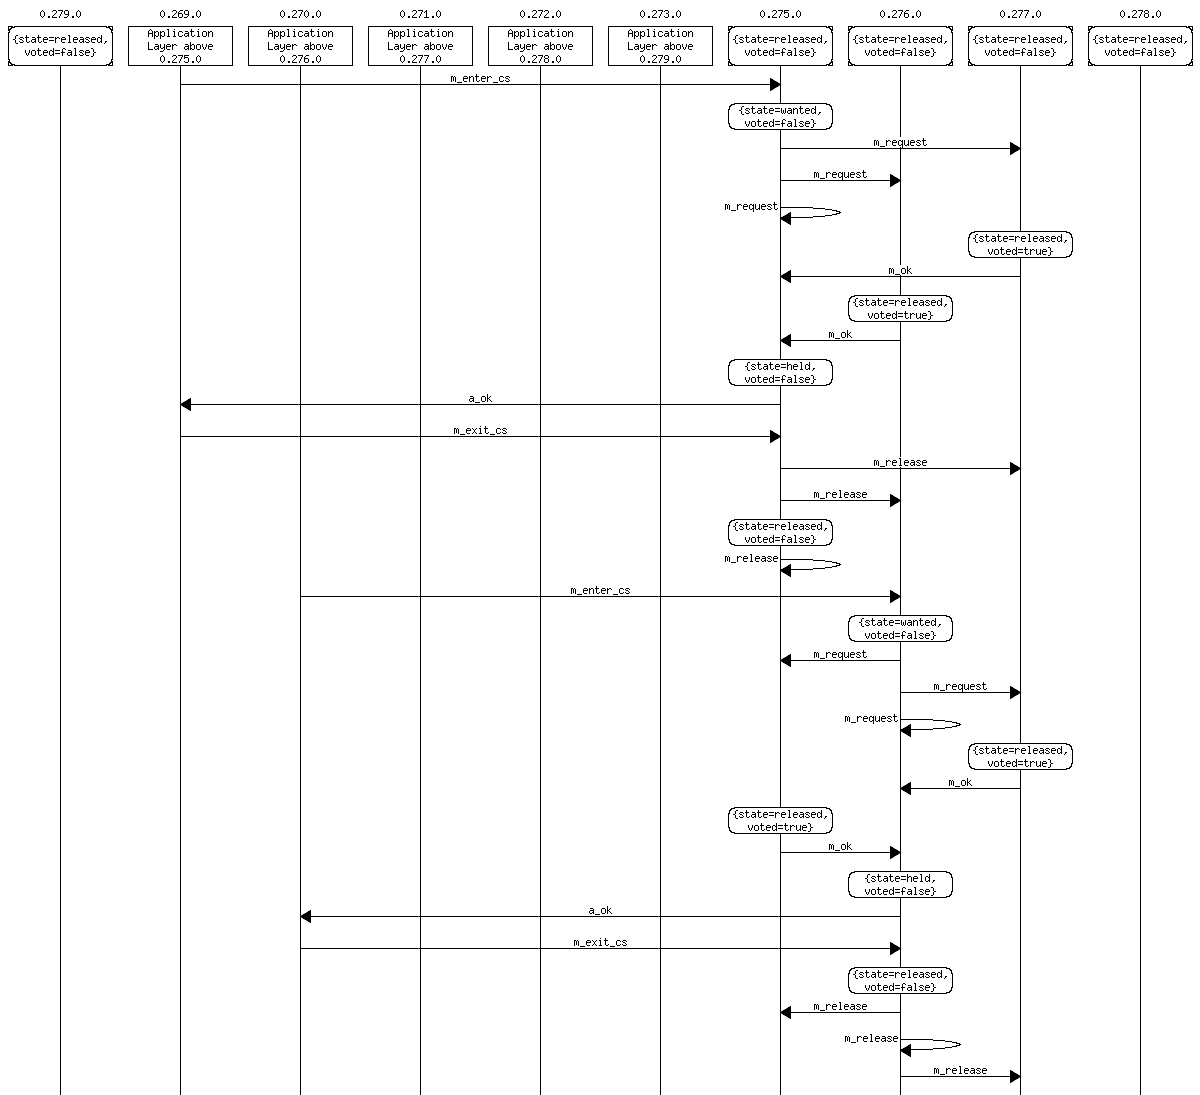
\includegraphics[scale=0.4]{../msc.png}
 \verbatiminput{../protokoll}

\section*{Erläuterungen}
 Das Programm wird mit dem Aufruf
 \begin{verbatim}
  ratemal:creator(Anzahl)
 \end{verbatim}
 gestartet.

 Das Programm ist in zwei Schichten implementiert, eine Anwendungdsschicht und
 eine darunter liegende Maekawaschicht.
 Die Einigung der Prozesse findet in der Maekawa-Schicht statt, die jeder
 Prozess für sich startet. An diese wird die Nachricht geschickt, dass der
 Prozess in die kritische Sektion eintretten will. Die Maekawa-Sschicht
 übernimmt das Aushandeln der Lockvergabe und das eventuelle Blockieren des
 entsprechenden Prozesses.
 \end{document}
